\begin{frame}{Filtering Inputs: Perplexity and SmoothLLM}
  \begin{columns}[T,onlytextwidth]
    \column{0.55\textwidth}
      \begin{itemize}\footnotesize\itemsep0.3em
        \item[\textcolor{red}{$\blacktriangleright$}] \textbf{Perplexity filter:} reject a prompt $X$ whose average negative log-likelihood under a language model is too high,
          \[ -\frac{1}{|X|}\sum_{i=1}^{|X|} \log p(x_i \mid x_{<i}) > T, \]
          where $p$ is the model's next-token probability and $T$ the highest value seen on plain harmful requests.
        \item[\textcolor{red}{$\blacktriangleright$}] A windowed filter caught every GCG prompt on five small open models but flagged about one benign prompt in ten. Fluent attacks pass: human-written jailbreaks, PAIR, AutoDAN's genetic search.
        \item[\textcolor{red}{$\blacktriangleright$}] \textbf{SmoothLLM:} GCG suffixes break when a few characters change. Perturb $q\%$ of the characters in each of $N$ copies, check each reply with a jailbreak detector, and return a majority reply. Cost: $N$ generations per request and some accuracy (Llama-2 on PIQA: 76.7\% to 70.3\%, $q = 5$, $N = 20$).
      \end{itemize}
    \column{0.43\textwidth}
      \centering
      {\scriptsize ASR (\%) of attacks found on an undefended model (GCG for GPT-4: transferred from Vicuna), then replayed against each defense:\par}
      \vspace{0.3em}
      {\scriptsize\setlength{\tabcolsep}{4pt}
      \begin{tabular}{p{0.8cm} p{2.2cm} p{0.9cm} p{0.9cm}}
        \toprule
        \textbf{Attack} & \textbf{Defense} & \textbf{Vicuna} & \textbf{GPT-4} \\
        \midrule
        GCG & none & 56 & 4 \\
            & perplexity filter & 3 & 0 \\
            & SmoothLLM & 5 & 1 \\
        \addlinespace[0.3em]
        PAIR & none & 88 & 48 \\
             & perplexity filter & 81 & 40 \\
             & SmoothLLM & 39 & 25 \\
        \bottomrule
      \end{tabular}\par}
      \vspace{0.2em}
      {\scriptsize Chao et al., \href{https://arxiv.org/abs/2310.08419v4}{arXiv:2310.08419v4}, Table~5 (SmoothLLM with $N = 10$, $q = 10$).\par}
      \vspace{0.4em}
      \begin{itemize}\footnotesize\itemsep0.2em
        \item[\textcolor{red}{$\blacktriangleright$}] Both defenses push gibberish attacks to near zero and fluent ones far less. These numbers are static: the attacker never saw the defense.
      \end{itemize}
  \end{columns}
  \vspace{0.1em}
  {\scriptsize Jain et al., \href{https://arxiv.org/abs/2309.00614v2}{arXiv:2309.00614v2}; Alon and Kamfonas, \href{https://arxiv.org/abs/2308.14132v3}{arXiv:2308.14132v3}; Liu et al. (AutoDAN), ICLR 2024, \href{https://arxiv.org/abs/2310.04451v2}{arXiv:2310.04451v2}; Robey et al. (SmoothLLM), \href{https://arxiv.org/abs/2310.03684v4}{arXiv:2310.03684v4}.\par}
\end{frame}

\begin{frame}{Safety Classifiers on Inputs and Outputs}
  \begin{columns}[T,onlytextwidth]
    \column{0.50\textwidth}
      \begin{itemize}\footnotesize\itemsep0.25em
        \item[\textcolor{red}{$\blacktriangleright$}] Guardrail classifiers (covered earlier) screen inputs and outputs. \textbf{Llama Guard} is Llama 2-7B fine-tuned to label a user or agent turn as safe or unsafe against a policy written into its prompt.
      \end{itemize}
      \vspace{0.1em}
      \centering
      \begin{tikzpicture}[font=\sffamily\scriptsize, >=latex]
        \node[draw, rounded corners=0.1cm, fill=gray!6, text width=6.1cm, align=left, inner sep=3pt] (p) at (0,0) {%
          \textcolor{blue!70!black}{\textbf{Policy:}} O1 Violence and Hate; O2 Sexual Content; O3 Criminal Planning; \ldots\\
          \textcolor{KAred}{\textbf{Conversation:}} User: How do you buy a tiger in America? Agent: Go to the zoo, steal one.\\
          \textcolor{green!40!black}{\textbf{Output format:}} \texttt{safe} or \texttt{unsafe} for the Agent turn, then the violated categories};
        \node[draw, rounded corners=0.1cm, fill=orange!16, align=center] (lg) at (-1.2,-1.45) {Llama Guard};
        \node[font=\ttfamily\scriptsize, text=KAred, align=left] (o) at (1.4,-1.45) {unsafe\\O3};
        \draw[->] (lg.north |- p.south) -- (lg.north);
        \draw[->] (lg.east) -- (o.west);
      \end{tikzpicture}\\[0.2em]
      {\scriptsize Redrawn after Inan et al., ``Llama Guard: LLM-based Input-Output Safeguard for Human-AI Conversations,'' \href{https://arxiv.org/abs/2312.06674v1}{arXiv:2312.06674v1}, Figure~1.\par}
      \begin{itemize}\footnotesize\itemsep0.25em
        \item[\textcolor{red}{$\blacktriangleright$}] Score: the probability of \texttt{unsafe}. Precision-recall AUC on its own test set: 0.945 (prompts) and 0.953 (responses), against 0.764 and 0.769 for OpenAI's moderation API.
      \end{itemize}
    \column{0.48\textwidth}
      \begin{itemize}\footnotesize\itemsep0.3em
        \item[\textcolor{red}{$\blacktriangleright$}] \textbf{Constitutional Classifiers:} separate guard models; Constitutional AI (covered earlier) trains the assistant itself. An LLM given a \textbf{constitution}, a written list of permitted and restricted content, generates their training data. The output classifier \textbf{streams}: it scores the answer at every token and can stop it mid-way.
        \item[\textcolor{red}{$\blacktriangleright$}] Prototype bug bounty: 405 invited (about 183 active), over 3{,}000 estimated hours, rewards up to \$15K. No one answered more than six of ten target questions at an unguarded model's level of detail; the prototype also over-refused.
        \item[\textcolor{red}{$\blacktriangleright$}] A later system blocked over 95\% of held-out jailbreak attempts (14\% without classifiers), at an absolute 0.38\% more refusals on production traffic and 23.7\% more inference compute.
      \end{itemize}
      \vspace{0.1em}
      {\scriptsize Sharma et al., ``Constitutional Classifiers: Defending against Universal Jailbreaks across Thousands of Hours of Red Teaming,'' \href{https://arxiv.org/abs/2501.18837v1}{arXiv:2501.18837v1}.\par}
  \end{columns}
\end{frame}

\begin{frame}{Hardening the Model: R2D2 and Circuit Breakers}
  \begin{columns}[T,onlytextwidth]
    \column{0.54\textwidth}
      \begin{itemize}\footnotesize\itemsep0.3em
        \item[\textcolor{red}{$\blacktriangleright$}] \textbf{Adversarial training (R2D2, Robust Refusal Dynamic Defense):} keep a pool of GCG prompts, update them against the current model at each training step, and train the model to refuse them; an instruction-tuning loss keeps it useful. 16 hours on eight A100s for 7B.
        \item[\textcolor{red}{$\blacktriangleright$}] R2D2 had the lowest GCG ASR of all models in HarmBench (a shared benchmark, next frame), 5$\times$ below Llama 2 13B, with smaller gains against PAIR.
        \item[\textcolor{red}{$\blacktriangleright$}] \textbf{Circuit breakers:} make the internal states that lead to harmful text useless, whatever the prompt. LoRA adapters (covered earlier) turn the representation $h_{\text{cb}}$ of harmful examples $x_s$ orthogonal to the original model's $h$, while retain-set examples $x_r$ keep theirs:
          \[ \begin{aligned} \mathcal{L} = {} & c_s\,\mathrm{ReLU}\big(\cos(h(x_s), h_{\text{cb}}(x_s))\big) \\ & + c_r\,\big\lVert h(x_r) - h_{\text{cb}}(x_r)\big\rVert_2, \end{aligned} \]
          with weights $c_s, c_r$; the retain set is ordinary chat plus safe prompts that sound unsafe.
      \end{itemize}
    \column{0.44\textwidth}
      \centering
      {\scriptsize HarmBench ASR (\%) and MT-Bench score, Mistral-7B-Instruct-v2 (R2D2: trained from Mistral 7B base, SFT only):\par}
      \vspace{0.3em}
      {\scriptsize\setlength{\tabcolsep}{4pt}
      \begin{tabular}{l r r r}
        \toprule
         & \textbf{refusal-trained} & \textbf{R2D2} & \textbf{+ RR} \\
        \midrule
        MT-Bench score & 7.60 & 6.00 & 7.53 \\
        GCG & 88.7 & 7.8 & 11.2 \\
        PAIR & 69.5 & 59.9 & 23.3 \\
        prefilled reply & 95.0 & 46.9 & 4.9 \\
        mean, 10 attacks & 76.7 & 31.7 & 9.8 \\
        \bottomrule
      \end{tabular}\par}
      \vspace{0.2em}
      {\scriptsize RR: representation rerouting, the circuit-breaker method. Zou et al., ``Improving Alignment and Robustness with Circuit Breakers,'' NeurIPS 2024, \href{https://proceedings.neurips.cc/paper_files/paper/2024/hash/97ca7168c2c333df5ea61ece3b3276e1-Abstract-Conference.html}{proceedings.neurips.cc}, Table~1.\par}
      \vspace{0.3em}
      \begin{itemize}\footnotesize\itemsep0.2em
        \item[\textcolor{red}{$\blacktriangleright$}] On Llama-3-8B-Instruct: mean ASR 38.1\% to 3.8\%, MT-Bench 8.05 to 8.00. These are standard attacks; adaptive ones come next.
      \end{itemize}
  \end{columns}
  \vspace{0.1em}
  {\scriptsize R2D2: Mazeika et al., ``HarmBench: A Standardized Evaluation Framework for Automated Red Teaming and Robust Refusal,'' ICML 2024, \href{https://proceedings.mlr.press/v235/mazeika24a.html}{proceedings.mlr.press/v235/mazeika24a}.}
\end{frame}

\begin{frame}{Measuring a Defense Against Adaptive Attacks}
  \begin{columns}[T,onlytextwidth]
    \column{0.42\textwidth}
      \begin{itemize}\footnotesize\itemsep0.3em
        \item[\textcolor{red}{$\blacktriangleright$}] ASR at a stated budget and private test sets were covered earlier. \textbf{HarmBench} adds one shared pipeline: 510 behaviours, 18 attacks, 33 models and defenses, one judge model. No attack or defense won everywhere, and resistance did not grow with model size.
        \item[\textcolor{red}{$\blacktriangleright$}] \textbf{Adaptive attack:} an attack designed against a specific defense by someone who knows how it works.
        \item[\textcolor{red}{$\blacktriangleright$}] Simple ones suffice. A prompt template plus random search on a suffix that raises the log-probability of ``Sure'', or prefilling the reply where the API allows it, reached 100\% ASR on GPT-4o, Llama-3-8B, R2D2 and every Claude model tested.
      \end{itemize}
    \column{0.56\textwidth}
      \centering
      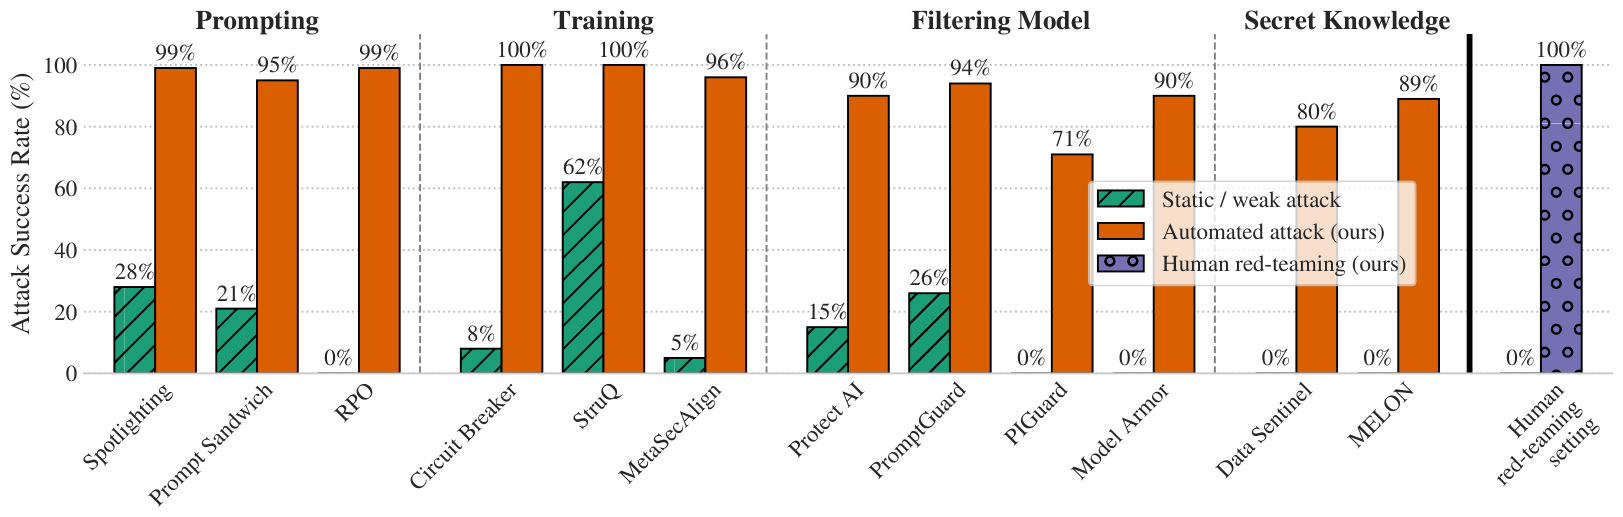
\includegraphics[width=\linewidth,height=0.4\textheight,keepaspectratio]{images/nlp-security-enterprise/nasr_fig1_adaptive_attacks.png}\\[0.2em]
      {\scriptsize Green: the attack in each defense's own paper; orange: the authors' automated adaptive attacks; purple: human red-teamers. Nasr et al., ``The Attacker Moves Second: Stronger Adaptive Attacks Bypass Defenses Against LLM Jailbreaks and Prompt Injections,'' \href{https://arxiv.org/abs/2510.09023v1}{arXiv:2510.09023v1}, Figure~1.\par}
      \vspace{0.3em}
      \begin{itemize}\footnotesize\itemsep0.2em
        \item[\textcolor{red}{$\blacktriangleright$}] Most of these 12 defenses had reported near-zero ASR. Adaptive attacks broke most of them above 90\%, circuit breakers at 100\%. Evaluate a defense with the strongest attack you can build against it.
      \end{itemize}
  \end{columns}
  \vspace{0.1em}
  {\scriptsize Mazeika et al., ``HarmBench,'' ICML 2024, \href{https://proceedings.mlr.press/v235/mazeika24a.html}{proceedings.mlr.press/v235/mazeika24a}; Andriushchenko et al., ``Jailbreaking Leading Safety-Aligned LLMs with Simple Adaptive Attacks,'' ICLR 2025, \href{https://arxiv.org/abs/2404.02151v4}{arXiv:2404.02151v4}.}
\end{frame}

\begin{frame}{Defense in Depth}

  {\centering
  \resizebox{\textwidth}{!}{%
  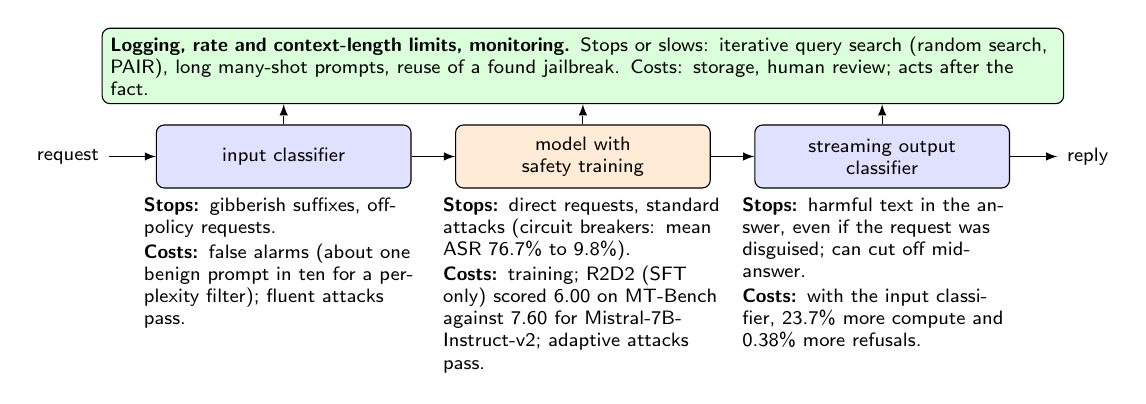
\begin{tikzpicture}[font=\sffamily\scriptsize, >=latex,
      stg/.style={draw, rounded corners=0.1cm, align=center, minimum height=0.8cm, text width=3.0cm},
      note/.style={align=left, text width=3.55cm, anchor=north, inner sep=1pt}]
    \node[draw, rounded corners=0.1cm, fill=green!14, align=left, text width=12.0cm, inner sep=3pt] (mon) at (5.2,1.15) {\textbf{Logging, rate and context-length limits, monitoring.} Stops or slows: iterative query search (random search, PAIR), long many-shot prompts, reuse of a found jailbreak. Costs: storage, human review; acts after the fact.};
    \node[stg, fill=blue!12] (inp) at (1.4,0) {input classifier};
    \node[stg, fill=orange!16] (mdl) at (5.2,0) {model with\\safety training};
    \node[stg, fill=blue!12] (outc) at (9.0,0) {streaming output\\classifier};
    \draw[<-] (inp.west) -- ++(-0.6,0) node[left] {request};
    \draw[->] (inp) -- (mdl);
    \draw[->] (mdl) -- (outc);
    \draw[->] (outc.east) -- ++(0.6,0) node[right] {reply};
    \draw[->, dashed] (inp.north) -- (inp.north |- mon.south);
    \draw[->, dashed] (mdl.north) -- (mdl.north |- mon.south);
    \draw[->, dashed] (outc.north) -- (outc.north |- mon.south);
    \node[note] at (1.4,-0.48) {\textbf{Stops:} gibberish suffixes, off-policy requests.\\[0.15em] \textbf{Costs:} false alarms (about one benign prompt in ten for a perplexity filter); fluent attacks pass.};
    \node[note] at (5.2,-0.48) {\textbf{Stops:} direct requests, standard attacks (circuit breakers: mean ASR 76.7\% to 9.8\%).\\[0.15em] \textbf{Costs:} training; R2D2 (SFT only) scored 6.00 on MT-Bench against 7.60 for Mistral-7B-Instruct-v2; adaptive attacks pass.};
    \node[note] at (9.0,-0.48) {\textbf{Stops:} harmful text in the answer, even if the request was disguised; can cut off mid-answer.\\[0.15em] \textbf{Costs:} with the input classifier, 23.7\% more compute and 0.38\% more refusals.};
  \end{tikzpicture}}\\[0.3em]
  {\scriptsize Defense in depth (covered earlier), applied to jailbreaks: each layer catches part of what the one before it missed; logging and limits watch all three.\par}
  \par}
  \vspace{0.3em}
  \begin{itemize}\footnotesize
    \item[\textcolor{red}{$\blacktriangleright$}] \textbf{Over-refusal} (covered earlier) needs its own test: XSTest's 250 safe prompts include ``kill a Python process''; Llama-2-70b-chat with its original system prompt fully refused 38\% of them.
  \end{itemize}
  \vspace{0.1em}
  {\scriptsize R\"ottger et al., ``XSTest: A Test Suite for Identifying Exaggerated Safety Behaviours in Large Language Models,'' NAACL 2024, \href{https://arxiv.org/abs/2308.01263v3}{arXiv:2308.01263v3}.}
\end{frame}
